\documentclass[aps,prl,twocolumn,reprint,amsmath,amssymb]{revtex4-1}

\usepackage{epsfig,color,graphicx}
\begin{document}
\newcommand{\Ang}{\ensuremath{\mathring{\text{A}}}}
\newcommand{\ltwid}{\mathrel{\raise.3ex\hbox{$<$\kern-.75em\lower1ex\hbox{$\sim$}}}}
\newcommand{\gtwid}{\mathrel{\raise.3ex\hbox{$>$\kern-.75em\lower1ex\hbox{$\sim$}}}}
\newcommand{\ket}[1]{\ensuremath{\vert #1 \rangle}}
\newcommand{\bra}[1]{\ensuremath{\langle #1 \vert}}
\newcommand{\braket}[2]{\ensuremath{\langle #1 \vert #2 \rangle}} % bra-ket inner product
\newcommand{\ketbra}[2]{\ensuremath{\vert #1 \rangle \langle #2 \vert}} % ket-bra outer product
\newcommand{\op}[1]{\ensuremath{\hat{#1}}} % operator
%\newcommand{\sill}{\psi_\mathrm{SILL}}
\newcommand{\sill}{\psi}
\newcommand{\trace}{{\rm Tr}}
\newcommand{\ntilde}{\tilde{n}}
\newcommand{\stilde}{\tilde{s}}
\newcommand{\atilde}{\tilde{\alpha}}
\newcommand{\new}{\color{red}}
\newcommand{\old}{\color{black}}
\newcommand{\bea}{\begin{eqnarray}}
\newcommand{\eea}{\end{eqnarray}}
\newcommand{\br}{\ensuremath{\mathbf{r}}}
\def\nn{\nonumber\\}

\bibliographystyle{apsrev}

\title{Supplementary Material:\\
Robust linear-scaling optimization of compact localized orbitals\\
in density functional theory}

\author{Yifei Shi}
\author{Rustam Z. Khaliullin}
\email{rustam.khaliullin@mcgill.ca}
\affiliation{Department of Chemistry, McGill University, 801 Sherbrooke St. West, Montreal, QC H3A 0B8, Canada}

\setcounter{equation}{0}
\setcounter{figure}{0}

\renewcommand{\theequation}{S\arabic{equation}}
\renewcommand{\thefigure}{S\arabic{figure}}


%%%$\bar{x}$-coefficients of the $y$-centered orbitals projected onto $\bar{x}$-space are determined by
%%%%
%%%\bea
%%%\op{I}_{\bar{x}} \ket{\psi_{yi}}  &=& \ket{\chi_{\bar{x}\mu}} S^{\bar{x}\mu,\bar{x}\nu} \braket{ \chi_{\bar{x}\nu}}{ \chi_{\bar{y}\lambda}}\, {T^{\bar{y}\lambda}}_{yi} = \nonumber \\
%%% &=& \ket{\chi_{\bar{x}\mu}} \left[ S^{\bar{x}\mu,\bar{x}\nu} S_{\bar{x}\nu,\bar{y}\lambda} {T^{\bar{y}\lambda}}_{yi} \right]
%%%\eea 
%%%}
%%%%
%%%Note that coefficients outside $\bar{x}$ may be nonzero but we do not need them.

\maketitle

\section{Relation between the Hessian and preconditioner}
 
The second derivative of the energy with respect to the CLMO coefficients is
%
\bea \label{eq:hessian}
{\Gamma_{\bar{x}\mu,\bar{y}\nu}}^{xi,yj} &\equiv & \frac{\partial^2 E}{\partial {T^{\bar{y}\nu}}_{yj} \partial {T^{\bar{x}\mu}}_{xi}} \nonumber \\ 
&=& 4 \bra{\chi_{\bar{x}\mu}} (\op{I}-\op{R}) \op{H} (\op{I}-\op{R}) \ket{\chi_{\bar{y}\nu}} \sigma^{yj,xi} - \nonumber \\
&-& 4 \bra{\chi_{\bar{x}\mu}} (\op{I}-\op{R}) \ket{\chi_{\bar{y}\nu}} \bra{\phi^{yj}} \op{H} \ket{\phi^{xi}} - \nonumber \\
&-& 4 \braket{\chi_{\bar{x}\mu}}{\phi^{yj}} \bra{\chi_{\bar{y}\nu}} (\op{I}-\op{R}) \op{H} \ket{\phi^{xi}} - \nonumber \\
&-& 4 \bra{\chi_{\bar{x}\mu}} (\op{I}-\op{R}) \op{H} \ket{\phi^{yj}} \braket{\chi_{\bar{y}\nu}}{\phi^{xi}} - \nonumber \\
&+& 4 \sum_{z,w} \bra{\chi_{\bar{x}\mu}} (\op{I}-\op{R}) \ket{\chi^{z\lambda}} \frac{\partial \op{H}_{z\lambda,w\kappa} }{\partial {T^{\bar{y}\nu}}_{yj}} \braket{\chi^{w\kappa}}{\phi^{xi}} \nonumber
%\right]
\eea 
%
The preconditioner defined in the main text is an approximation to this Hessian. The preconditioner is evaluated only within the same domain (i.e. $y=x$) with the T-dependence of the Kohn-Sham Hamiltonian and, thus, the last term neglected. Additionally, the $\sigma^{xj,xi}$ is approximated with the identity matrix and $\bra{\phi^{xj}} \op{H} \ket{\phi^{xi}}$ is set to $-\delta_{ji}$. The third and fourth terms are also neglected because, for $x=y$, they contain the gradient, which becomes small as the ground state is approached in the iterative procedure.

\section{Eigenvalues of the preconditioner} 

Figure~\ref{sfig:hesseig} shows the eigenvalues of the preconditioner for several cases in a typical calculation. For completely delocalized orbitals, the eigenvalues are either exactly zero (occupied-occupied mixing) or very large (occupied-virtual mixing). For the straightforward optimization of CLMOs, the eigenvalue spectrum is continuous and low-curvature modes exist. For the optimization with the low-curvature projector (LCP) and $\Lambda_{c}=RZK$~a.u., the small and large eigenvalues are again separated. %after removing some of the small eigenvectors.

\begin{figure}[t!]
\centering
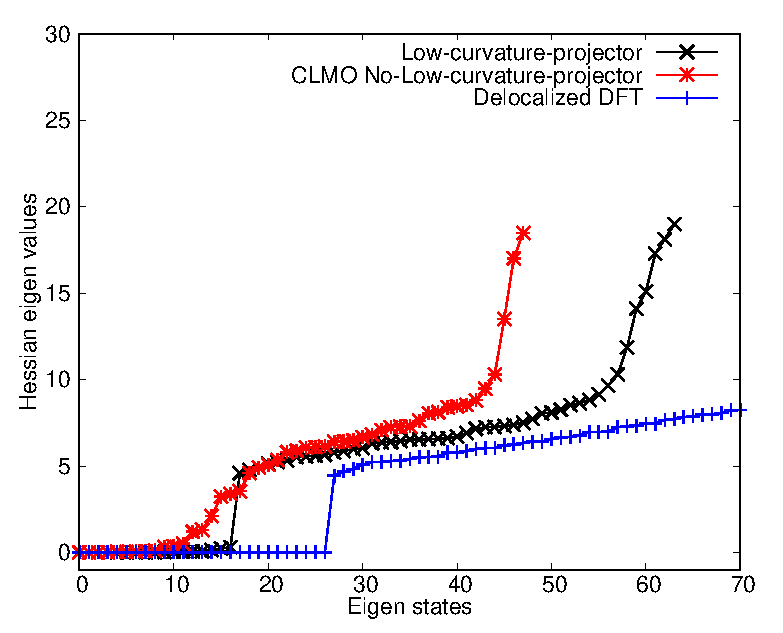
\includegraphics[width=0.4\textwidth]{Hesseig}
\caption{Eigenvalues of the preconditioner in the final stages of the PBE/DZVP orbital optimization for hexagonal CdSe lattice with eight atoms. To display the zero eigenvalues on the logarithmic scale, all eigenvalues values are shifted up by $10^{-RZK}$~a.u. For the CLMO optimization, the localization domain includes the central Cd$^{2+}$ ion and three Se$^{2-}$ ions. For the delocalized orbitals, the domain includes the entire system and only low eigenvalues are shown. For the CLMO optimization without the low-curvature projector, the calculation does not converge and the preconditioner is evaluated at final iterations, for which the energy is close to the ground state.}
%RZK "Hessian eigen values" -> "Eigenvalues, a.u." 
%RZK "Delocalized DFT" -> "Delocalized orbitals"
%RZK "CLMO No-Low-curvature-projector" -> "CLMO without LCP"
%RZK "Low-curvature-projector" -> "CLMO with LCP"
%RZK Use y-log scale. To display zero eigenvalues add a small epsilon to all eigenvalues. 
\label{sfig:hesseig}
\end{figure}

\section{Physical origin of the low-curvature modes}

In the main text, we suggested that the low-curvature optimization modes represent occupied-hybrid mixing modes, where the hybrid states are mostly but not completely occupied. 
These occupied-hybrid modes directions exist in the vector space of domain $\bar{x}$ because CLMOs of the neighbor centers are not completely localized on $\bar{x}$. 
Our hypothesis implies that a hybrid low-curvature mode $\ket{d_{\bar{x}p}}$ has only small component in the unoccupied subspace of domain $\bar{x}$. 
This component is measured by the residue $\Delta_{\bar{x}p}$ 
%
\bea
%\label{eq:residue}
\Delta_{\bar{x}p} \equiv \bra{d_{\bar{x}p}} \op{I}_{\bar{x}} - \op{R}_{\bar{x}} \ket{d_{\bar{x}p}}, 
\eea
%
where $\op{R}_{\bar{x}}$ is a projector constructed from the occupied CLMOs of the neighbors truncated to the subspace $\bar{x}$ with operator $\op{T}_{\bar{x}} \approx \op{I}_{\bar{x}}$
%
\bea
\op{R}_{\bar{x}} &=& \sum_{y,z \in \bar{x}} \op{T}_{\bar{x}} \ket{\psi_{yi}} \sigma_{\bar{x}}^{yi,zj} \bra{\psi_{zj}} \op{T}_{\bar{x}}
%\label{eq:C}
\eea
%
and $\sigma_{\bar{x}}$ is the overlap matrix of the truncated orbitals. 

Unfortunately, it is difficult to unambiguously divide the vector space of a domain into the occupied $\op{R}_{\bar{x}}$ and unoccupied $(\op{I}_{\bar{x}} - \op{R}_{\bar{x}})$ subspaces because of substantial electron delocalization between centers (i.e. atoms). 
In our definition, the unoccupied subspace is ultimately determined by what orbitals are included into projector $\op{R}_{\bar{x}}$. 

Here, we discuss the dependence of residues $\Delta$ on dimensionless parameter $t \in [0,1]$ -- a proxy for the tunable size of the \emph{occupied} subspace of $\bar{x}$. First, we introduce a measure of what fraction of a normalized CLMO $\ket{\psi_{yj}}$ is present outside domain $\bar{x}$:
\bea
M^{\bar{x}}_{yj} \equiv \bra{\psi_{yj}} (\op{I} - \op{I}_{\bar{x}}) \ket{\psi_{yj}}
\eea
%
% RZK: state \ket{\psi_{yj}} should be normalized
Second, we include only those $\ket{\psi_{yi}}$ states into $\op{R}_{\bar{x}}$ whose presence outside $\bar{x}$ is below
\bea
M^{\bar{x}}_{yj} < t
\eea
%
where cutoff threshold $t \in [0,1]$. 
For example, $t = 0.2$ means that $\op{R}_{\bar{x}}$ includes the orbitals, whose presence on $\bar{x}$ is 80\% or more. 
For larger $t$, more and more states outside $\bar{x}$ are included into $\op{R}_{\bar{x}}$ thus reducing the dimension of the unoccupied space on $\bar{x}$ and, as a consequence, bringing $\Delta$ down.

The dependence of $\Delta$ on $t$ for the materials described in main-text is shown in Figures~\ref{sfig:t_delta_tio2}--\ref{sfig:t_delta_si}. 
The assumption that the low-curvature modes have small presence in the unoccupied space holds for TiO$_2$, CdSe, water cluster with atomic partitioning. However, it is less accurate for Si where optimal CLMOs are less localized.

\begin{figure}
\centering
\includegraphics[width=0.3\textwidth]{t_tio2_residue}
\caption{$\Delta$ as a function of $t$ for Ti$^{4+}$ ions in the TiO$_2$ rutile lattice.}
\label{sfig:t_delta_tio2}
\end{figure}

\begin{figure}
\centering
\includegraphics[width=0.3\textwidth]{t_cdse_residue}
\caption{$\Delta$ as a function of $t$ for Cd$^{2+}$ ions in the CdSe Wurtzite lattice.}
\label{sfig:t_delta_cdse}
\end{figure}

\begin{figure}
\centering
\includegraphics[width=0.3\textwidth]{t_water_residue}
\caption{$\Delta$ as a function of $t$ for O$^{2-}$ in water tetramer.}
\label{sfig:t_delta_water}
\end{figure}

\begin{figure}
\centering
\includegraphics[width=0.3\textwidth]{t_si_residue}
\caption{$\Delta$ as a function of $t$ for Si atom in the diamond silicon lattice.}
\label{sfig:t_delta_si}
\end{figure}




%\begin{figure}
%\centering
%\includegraphics[width=0.3\textwidth]{t_tio2_residue}
%\includegraphics[width=0.3\textwidth]{t_cdse_residue}
%\includegraphics[width=0.3\textwidth]{t_water_residue}
%\includegraphics[width=0.3\textwidth]{t_si_residue}
%\caption{$\Delta$ as a function of $t$ for: Ti$^{4+}$ ions in the TiO$_2$ rutile lattice, Cd$^{2+}$ ions in the CdSe Wurtzite lattice, O$^{2-}$ in water tetramer, Si atom in the diamond silicon lattice.}
%\label{sfig:t_delta}
%\end{figure}
%

\end{document}
